\documentclass[11pt]{article}

% some definitions for the title page
\newcommand{\reporttitle}{example}
\newcommand{\reportdescription}{example description}

% load some definitions and default packages
%---------------------------------------------------------------------------
%	PACKAGES AND OTHER DOCUMENT CONFIGURATIONS
%---------------------------------------------------------------------------

\usepackage[twoside]{fancyhdr}
\usepackage{csquotes}

\usepackage[a4paper,hmargin=2.0cm,vmargin=1.0cm,includeheadfoot]{geometry}
% \usepackage{natbib} % for bibliography
\usepackage{biblatex}
\usepackage{tabularx,longtable,multirow,subfigure,caption}%hangcaption
\usepackage{fancyhdr} % page layout
\usepackage{url} % URLs
\usepackage[english]{babel}
\usepackage{graphicx}
\usepackage{rotating}
\usepackage{dsfont}
\usepackage{epstopdf} % automatically replace .eps with .pdf in graphics
% \usepackage{backref} % needed for citations
\usepackage{array}
\usepackage{latexsym}
\usepackage[pdftex,hypertexnames=false,colorlinks]{hyperref} % provide links in pdf (had pagebackref)
\usepackage{booktabs}
\usepackage{wrapfig}
\usepackage{caption}  % Required for \captionof
\usepackage{float} % for H option in figures
\usepackage{amssymb}
\usepackage{amsmath}
\usepackage{amsthm}
\usepackage{mathtools} % for 'dcases*' env.
\usepackage[nottoc]{tocbibind}

%%% Default fonts
\renewcommand*{\rmdefault}{bch}
\renewcommand*{\ttdefault}{cmtt}

%%% Default settings (page layout)
\setlength{\parindent}{0em}  % indentation of paragraph
\setlength{\parskip}{.3em}
\setlength{\itemsep}{0.mm}

\setlength{\headheight}{14.5pt}
\pagestyle{fancy}

\fancyfoot[ER,OL]{\thepage}%Page no. in the left on odd pages and on right on even pages

\fancyfoot[OC,EC]{\sffamily }
\renewcommand{\headrulewidth}{0.1pt}
\renewcommand{\footrulewidth}{0.1pt}
\captionsetup{margin=10pt,font=small,labelfont=bf}

% LISTINGS ammendments
\usepackage{listings}
\usepackage{color}

\definecolor{mygreen}{rgb}{0,0.6,0}
\definecolor{mygray}{rgb}{0.5,0.5,0.5}
\definecolor{mymauve}{rgb}{0.58,0,0.82}

\lstset{ 
  postbreak=\mbox{\textcolor{red}{$\hookrightarrow$}\space},
  backgroundcolor=\color{white},   % choose the background color; you must add \usepackage{color} or \usepackage{xcolor}; should come as last argument
  basicstyle=\footnotesize,        % the size of the fonts that are used for the code
  breakatwhitespace=false,         % sets if automatic breaks should only happen at whitespace
  breaklines=true,                 % sets automatic line breaking
  captionpos=b,                    % sets the caption-position to bottom
  commentstyle=\color{mygreen},    % comment style
%   deletekeywords={...},            % if you want to delete keywords from the given language
%   escapeinside={\%*}{*)},          % if you want to add LaTeX within your code
  extendedchars=true,              % lets you use non-ASCII characters; for 8-bits encodings only, does not work with UTF-8
  firstnumber=1,                % start line enumeration with line 1000
  frame=single,	                   % adds a frame around the code
  keepspaces=true,                 % keeps spaces in text, useful for keeping indentation of code (possibly needs columns=flexible)
  columns=fullflexible,
  keywordstyle=\color{blue},       % keyword style
  language=python,                 % the language of the code
  % morekeywords={*,...},            % if you want to add more keywords to the set
  numbers=left,                    % where to put the line-numbers; possible values are (none, left, right)
  numbersep=5pt,                   % how far the line-numbers are from the code
  numberstyle=\tiny\color{mygray}, % the style that is used for the line-numbers
  rulecolor=\color{black},         % if not set, the frame-color may be changed on line-breaks within not-black text (e.g. comments (green here))
  showspaces=false,                % show spaces everywhere adding particular underscores; it overrides 'showstringspaces'
  showstringspaces=false,          % underline spaces within strings only
  showtabs=false,                  % show tabs within strings adding particular underscores
  stepnumber=1,                    % the step between two line-numbers. If it's 1, each line will be numbered
  stringstyle=\color{mymauve},     % string literal style
  tabsize=2,	                   % sets default tabsize to 2 spaces
  title=\lstname% show the filename of files included with \lstinputlisting; also try caption instead of title
}

% Here, you can define your own macros. Some examples are given below.

\newcommand{\R}[0]{\mathds{R}} % real numbers
\newcommand{\Z}[0]{\mathds{Z}} % integers
\newcommand{\N}[0]{\mathds{N}} % natural numbers
\newcommand{\C}[0]{\mathds{C}} % complex numbers
\renewcommand{\vec}[1]{{\boldsymbol{{#1}}}} % vector
\newcommand{\mat}[1]{{\boldsymbol{{#1}}}} % matrix


%\bibliography{bibliography}

\begin{document}

% Include the title page
\begin{titlepage}

    \newcommand{\HRule}{\rule{\linewidth}{0.5mm}} % Defines a new command for the horizontal lines, change thickness here
    
    \center % Center everything on the page
     
    %------------------------------------------------------------------------
    %	HEADING SECTIONS
    %------------------------------------------------------------------------
    
    \textsc{\Large Department of Computing}\\[0.5cm] 
    \textsc{\large Imperial College of Science, Technology and Medicine}\\[0.5cm] 
    
    %------------------------------------------------------------------------
    %	TITLE SECTION
    %------------------------------------------------------------------------
    
    \HRule \\[0.4cm]
    { \huge \bfseries \reporttitle}\\ % Title of your document
    \HRule \\[0.4cm]

    \textit{\reportdescription}
    
    \vspace{2em}

    %------------------------------------------------------------------------
    %	AUTHOR SECTION
    %------------------------------------------------------------------------
    
    \large \emph{Author: Anton Zhitomirskiy}

    \vspace{1em}

    \global\let\newpagegood\newpage
    \global\let\newpage\relax
    
\end{titlepage}

\global\let\newpage\newpagegood

\tableofcontents

\clearpage

\section{Sparsity}

\subsection{Problem}

If certain words are absent then the proability in the n-gram is zero. We can use smoothing to solve this or give it unknown word tokens. 
% Alternatively, we can give an unknown word token (but these have to be in the training set and the test set). This unknown word is used if a word appears to little times, or we apply this directly to our vocabulary set.

\subsection{Add-one smoothing}

\begin{figure}[H]
    \centering
    \subfigure[Counts after one-smoothing (we've added +1 to EVERYTHING)]{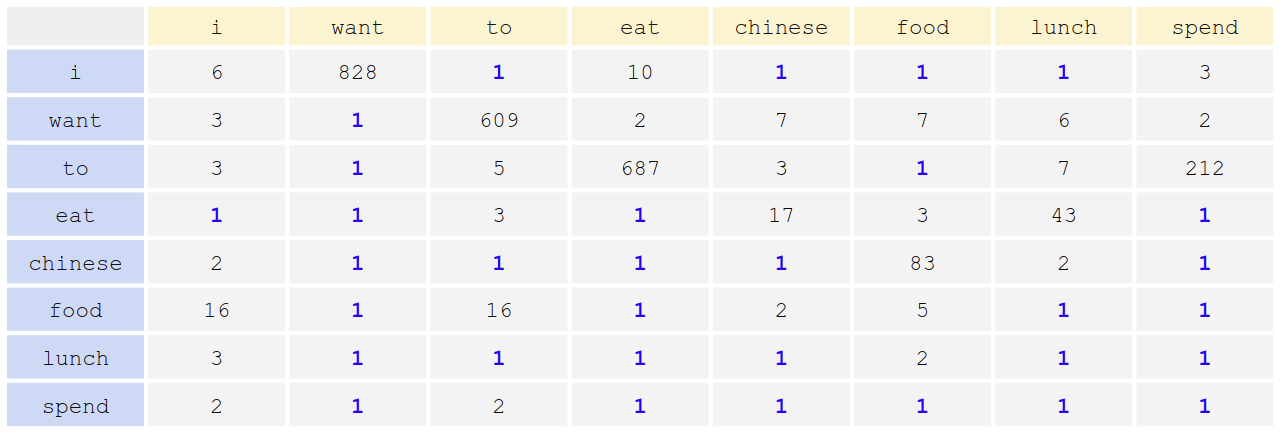
\includegraphics[width=.8\linewidth]{figures/after-one-smoothing.png}}
    \subfigure[probabilities before one-smoothing]{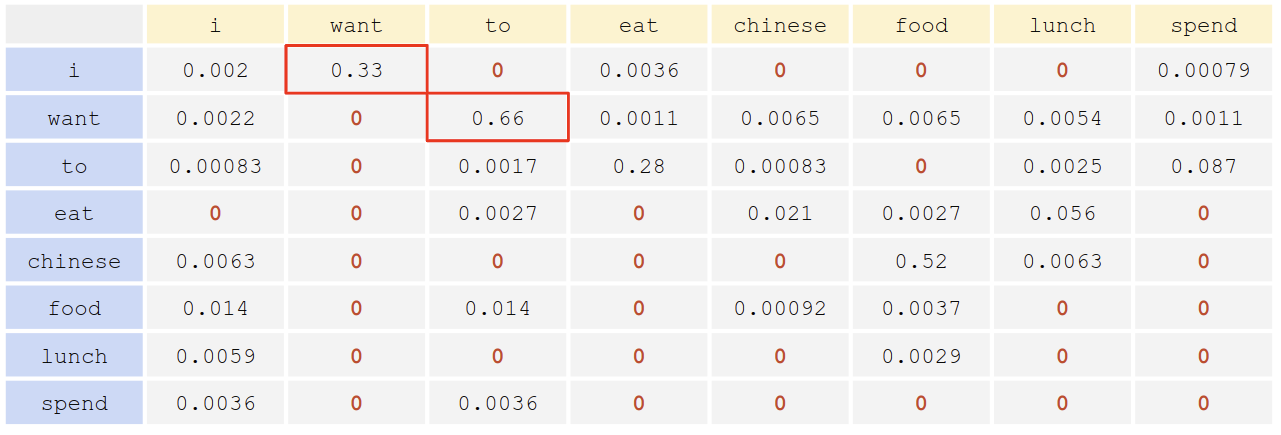
\includegraphics[width=.8\linewidth]{figures/before-one-smoothing.png}}
    \subfigure[probabilities after one-smoothing]{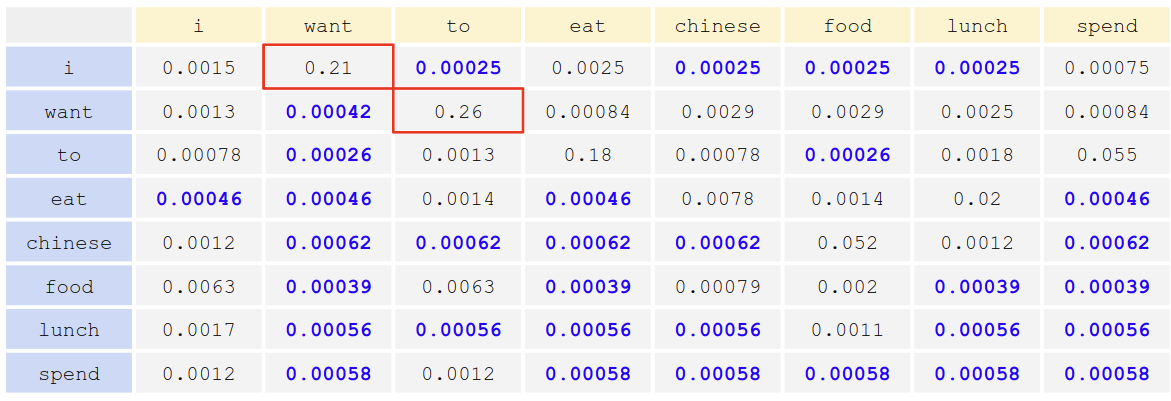
\includegraphics[width=.8\linewidth]{figures/after-one-smoothing-probs.png}}
    \subfigure[total instances of words]{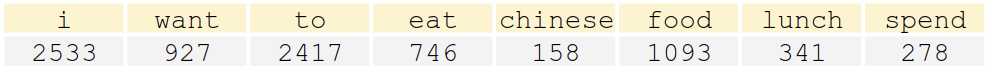
\includegraphics[width=.8\linewidth]{figures/bi-gram-total.png}}
    \caption{difference between smoothing and not}\label{fig:smoothing-example}
\end{figure}

\begin{equation*}
    P_{add-1}(w_n|w_{n-1})=\frac{C(w_{n-1},w_n)+1}{C(w_{n-1})+V}
\end{equation*}

Given words with sparse statistics, they steal probability mass from more frequent words. This is because smaller instances of vocabulary are more influenced by the V and +1 term appearing in the new fraction. However, for larger occurrences they shrink because the nominator is large (so +1) won't change it by much, but the denominator grows larger, making the overall probability less.

The change here is great between the hilighted terms in Figure~\ref{fig:smoothing-example}. ``If we have very few instances of the word `want' the smoothing will impact this a lot and this number will therefore change a lot. Wheras, if we have a lot of counts within the word `i' then it wont change the probability a lot.'' Indeed, looking at the total instances of word i, the denominator is so large already that the number wasn't impacted, and `want' was impacted.

\subsubsection{Problems}

Although easy to implement, it takes too much probability mass from more likely occurrences (see Figure~\ref{fig:smoothing-example}) and assigns too much probability to unseen events. Therefore, we could try +k smoothing witha  smaller value of k.

\subsection{Back-off smoothing}

If we don't have any occurrences in our current (trigram) model, we can back-off and see how many occurrences there are in the smaller (bigram) model.

\begin{definition}[Back off smoothing ``sutpid back-off'']
    \begin{align*}
        S(w_i|w_{i-2}w_{i-1}) &=
        \begin{cases}
            \frac{C(w_{i-2}w_{i-1}w_i)}{C(w_{i-2}w_{i-1})} , & if\ C(w_{i-2}w_{i-1}w_i) > 0 \\
            0.4 \cdot S(w_i|w_{i-1}) , & otherwise    
        \end{cases} \\
        S(w_i|w_{i-1}) &=
        \begin{cases}
            \frac{C(w_{i-1}w_i)}{C(w_{i-1})} , & if\ C(w_{i-1}w_i) > 0 \\
            0.4 \cdot S(w_i) , & otherwise    
        \end{cases} \\
        s(w_i) &= \frac{C(w_i)} N
    \end{align*}    
\end{definition}

Where $N$ is the number of words in the text

\subsubsection{Problems}

suppose that the bigram ``a b'' and the unigram ``c'' are very common, but the trigram ``a b c'' is never seen. Since ``a b'' and ``c'' are very common, it may be significant (that is, not due to chance) that ``a b c'' is never seen.

Perhaps it's not allowed by the rules of the grammar.  Instead of assigning a more appropriate value of 0, the method will back off to the bigram and estimate $P(c | b)$, which may be too high

\subsection{Interpolation}

Combine evidence from different n-grams:

\begin{definition}[Interpolation]
    \begin{equation*}
        P_{interp}(w_i|w_{i-2}w_{i-1})=\lambda_1 P(w_i|w_{i-2} w_{i-1}) + \lambda_2 P(w_i|w_{i-1}) + \lambda_3 P(w_i), \quad where\ \lambda_1 + \lambda_2 + \lambda_3 = 1
    \end{equation*}
\end{definition}

\section{Feed-forward neural language models}

\section{Vanilla RNNs for language modelling}

\section{Bi-directional RNNs}

\section{LSTMs and GRUs}

\section{Revision \& little tangent on de-biasing}

% \printbibliography
% \addcontentsline{toc}{section}{Bibliography}

\end{document}